\chapter{Improving Information Discovery and Curation Activities}
\label{chapter:improving}


\begin{figure}[ht!]
	\noindent
	\centering
	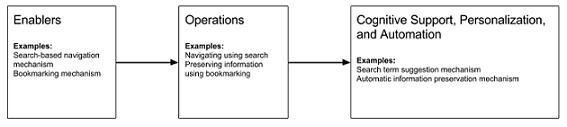
\includegraphics[width=\linewidth]{framework_part2.png}
	\caption{Framework Overview (Part II): Improving Information Discovery and Curation}
	\label{fig:framework_part2} 
\end{figure}

{\section{Improving Navigation}
There are two common ways of aiding information discovery when search-based navigation is used. The first method entails returning personalized results when the user enters a search query. There are a number of ways to accomplish personalization, but this chapter only focuses on which features can can support information discovery and curation have rather than their implementations. The second method is to suggest search terms to make it easier for the user to formulate the information need (see Table~\ref{table:navigation_support}).

To further support referential navigation, applications can either personalize search results (similarly to descriptional navigation) or personalize reference suggestions (see Table~\ref{table:navigation_support}). 

To further enhance random navigation, Web tools sometimes allow users to personalize this type of navigation, which makes it less 'random'. However, this way the user can discover new information within a specific category, for example.

Displayed content can also be personalized to improve information discovery with direct navigation.

\begin{table}[ht!]
\caption{Cognitive Support, Automation, and Personalization for Navigation}
\label{table:navigation_support}
\begin{tabular}{{|p{0.35\linewidth}|p{0.60\linewidth}|}}
\hline
Support, automation, and personalization elements & Questions to be posed during the design or evaluation of discovery and curation tools \\
\hline
\textbf{Descriptional}       & \\
Personalized results         & Does the search mechanism return personalized results? \\
Filtered search mechanism    & Is it possible to apply filters to the search criteria? \\
Guided search                & Does the system suggest search terms to the user? \\
\textbf{Referential}         & \\
Suggesting categories & Does the system suggest categories of interest? \\
Suggesting topics of interest & Does the system suggest topics of interest? \\
Suggesting tags              & Does the system suggest similar tags? \\
Suggesting similar resources & Does the system suggest similar resources? \\
\textbf{Opportunistic} & \\
Personalized opportunistic navigation     & Is it possible to personalize opportunistic navigation? \\
\textbf{System-regulated} & \\
Personalized featured content         & Is featured content personalized to the user? \\                                                       
User activity update notification & Is it possible to receive notifications about other users' activities? \\
Application activity update notification & Is it possible to receive notifications about website content updates?\\
Artifact update notification & Is it possible to receive notifications about artifact-related updates? \\                                                       
\hline

\end{tabular}
\end{table}


} % end subsection
{\section{Improving Exploration}

\begin{table}[ht!]
\caption{Visual and Spatial Exploration Cognitive Support and Personalization}
\begin{tabular}{{|p{0.33\linewidth}|p{0.62\linewidth}|}}
\hline
Cognitive support and personalization design elements & Questions to be posed during the design or evaluation of discovery and curation tools  \\
\hline
&\\
\textbf{Visual and textual cues of multiple resources} & \\
Personalized visual preview  & Is it possible to personalize visual previews of resources? \\
Personalized textual preview & Is it possible to personalize textual previews of resources? \\
&\\
\textbf{Visual and textual cues of a single resource} & \\
Personalized visual cues                 & Is it possible to personalize the visual cues within a resource? \\
Personalized textual cues                & Is it possible to personalize the textual cues within a resource? \\
&\\
\textbf{Spatial proximal cues of multiple resources} & \\
Personalized arrangement of multiple resources & Is it possible to personalize the arrangement of resources? \\   
&\\                                                 
\textbf{Spatial proximal cues of a single resource} & \\
Personalized arrangement of information within a resource          & Is it possible to personalize the arrangement of information within a resource? \\                                                       
\hline
\end{tabular}
\end{table}

} % end subsection

{\section{Improving Curation}

\begin{table}[ht!]
\caption{Cognitive Support, Personalization, and Automation for Curation}
\label{table:curation_support}
\begin{tabular}{{|p{0.30\linewidth}|p{0.65\linewidth}|}}
\hline
Cognitive support, personalization, and automation elements & Questions to be posed during the design or evaluation of information discovery and curation tools \\
\hline
\textbf{Management}		& \\
Suggesting collections  & Does the system suggest relevant collections? \\
Suggesting tags         & Does the system suggest relevant tags? \\
Automated classification into collections  	& Does the system automatically sort resources into collections? \\
Automated tagging       & Does the system automatically tag resources? \\
\textbf{Preservation}   & \\
History       			& Does the system automatically preserve information found by the user? \\
Suggested preservation  & Does the system suggest preservation channels to the user? \\
\textbf{Augmentation} 	& \\
Automated augmentation  & Does the system automatically annotate resources? \\
Suggested augmentation  & Does the system suggest annotation options to the user? \\    
\textbf{Sharing}        & \\
Automated sharing		&  Does the system support automatic sharing? \\
\textbf{Subscription}   & \\
Suggesting users for subscription & Does the system suggest which users to subscribe to? \\
Suggesting artifacts for subscription   & Does the system suggest which artifacts to subscribe to? \\
Automatic subscription  & Can the system subscribe the user automatically to the website activity? \\

\hline  
\end{tabular}
\end{table}
} % end subsection

{\section{Personalization Strategies}
} % end subsection

Providing cognitive support, personalization, and automation dramatically improves user experience when they interact with information discovery and curation systems. 